% ****** Start of file apssamp.tex ******
%
%   This file is part of the APS files in the REVTeX 4.1 distribution.
%   Version 4.1r of REVTeX, August 2010
%
%   Copyright (c) 2009, 2010 The American Physical Society.
%
%   See the REVTeX 4 README file for restrictions and more information.
%
% TeX'ing this file requires that you have AMS-LaTeX 2.0 installed
% as well as the rest of the prerequisites for REVTeX 4.1
%
% See the REVTeX 4 README file
% It also requires running BibTeX. The commands are as follows:
%
%  1)  latex apssamp.tex
%  2)  bibtex apssamp
%  3)  latex apssamp.tex
%  4)  latex apssamp.tex
%
\documentclass[%
%reprint,
%superscriptaddress,
%groupedaddress,
%unsortedaddress,
%runinaddress,
%frontmatterverbose, 
preprint,
%showpacs,preprintnumbers,
%nofootinbib,
%nobibnotes,
%bibnotes,
 amsmath,amssymb,
 aps,
%pra,
%prb,
%rmp,
%prstab,
%prstper,
%floatfix,
10.5pt,
]{revtex4-1}

\usepackage{graphicx}% Include figure files
\usepackage{subfigure}
\usepackage{multirow}
\usepackage{array}
\usepackage{dcolumn}% Align table columns on decimal point
\usepackage{bm}% bold math
%\usepackage{hyperref}% add hypertext capabilities
%\usepackage[mathlines]{lineno}% Enable numbering of text and display math
%\linenumbers\relax % Commence numbering lines

%\usepackage[showframe,%Uncomment any one of the following lines to test 
%%scale=0.7, marginratio={1:1, 2:3}, ignoreall,% default settings
%%text={7in,10in},centering,
%%margin=1.5in,
%%total={6.5in,8.75in}, top=1.2in, left=0.9in, includefoot,
%%height=10in,a5paper,hmargin={3cm,0.8in},
%]{geometry}

\usepackage{xeCJK}
%\setCJKmainfont[ItalicFont={KaiTi}, BoldFont={KaiTi}]{KaiTi}
\usepackage{textcomp}
\usepackage{chemfig}
\usepackage[version=4]{mhchem}
\usepackage{fontspec}
\usepackage{listings}
\usepackage{xcolor}
\usepackage{xcolor} % 定制颜色
\definecolor{mygreen}{rgb}{0,0.6,0}
\definecolor{mygray}{rgb}{0.5,0.5,0.5}
\definecolor{mymauve}{rgb}{0.58,0,0.82}
\lstset{
backgroundcolor=\color{white},      % choose the background color
basicstyle=\footnotesize\ttfamily,  % size of fonts used for the code
columns=fullflexible,
tabsize=4,
breaklines=true,               % automatic line breaking only at whitespace
captionpos=b,                  % sets the caption-position to bottom
commentstyle=\color{mygreen},  % comment style
escapeinside={\%*}{*)},        % if you want to add LaTeX within your code
keywordstyle=\color{blue},     % keyword style
stringstyle=\color{mymauve}\ttfamily,  % string literal style
frame=single,
rulesepcolor=\color{red!20!green!20!blue!20},
% identifierstyle=\color{red},
language=Mathematica,
}

\usepackage[normalem]{ulem}

\newcommand{\chuhao}{\fontsize{42pt}{44.9pt}\selectfont}    % 初号, 1.5倍行距
\newcommand{\xiaochu}{\fontsize{30pt}{40pt}\selectfont}    % 小初, 1.5倍行距
\newcommand{\yihao}{\fontsize{26pt}{36pt}\selectfont}    % 一号, 1.4倍行距
\newcommand{\erhao}{\fontsize{22pt}{28pt}\selectfont}    % 二号, 1.25倍行距
\newcommand{\xiaoer}{\fontsize{18pt}{18pt}\selectfont}    % 小二, 单倍行距
\newcommand{\sanhao}{\fontsize{16pt}{24pt}\selectfont}    % 三号, 1.5倍行距
\newcommand{\xiaosan}{\fontsize{15pt}{22pt}\selectfont}    % 小三, 1.5倍行距
\newcommand{\sihao}{\fontsize{14pt}{21pt}\selectfont}    % 四号, 1.5倍行距
\newcommand{\sihaox}{\fontsize{14pt}{28pt}\selectfont}    % 四号, 1.5倍行距
\newcommand{\banxiaosi}{\fontsize{13pt}{19.5pt}\selectfont}    % 半小四, 1.5倍行距
\newcommand{\xiaosix}{\fontsize{12pt}{24pt}\selectfont} 	% 小四, 1.5倍行距
\newcommand{\xiaosi}{\fontsize{12pt}{18pt}\selectfont}     
\newcommand{\dawuhao}{\fontsize{11pt}{11pt}\selectfont}    % 大五号, 单倍行距
\newcommand{\wuhao}{\fontsize{10.5pt}{10.5pt}\selectfont}    % 五号, 单倍行距
\newcommand{\xiaowu}{\fontsize{9pt}{9pt}\selectfont}    % 五号, 单倍行距

%\usepackage[fntef]{ctexcap}
%\CTEXsetup[number={\chinese{section}、},format={\Large\bfseries}]{section}
%\setCJKfamilyfont{fangsong}{FangSong}                      %仿宋2312 fs  
%\newcommand{\fangsong}{\CJKfamily{fangsong}}  

\usepackage{wrapfig}
\usepackage{fancyhdr}
\usepackage{fancybox}   


\usepackage{tikz}
\usepackage{circuitikz}



\newcommand{\bra}[1]{\langle #1 |}
\newcommand{\ket}[1]{| #1 \rangle}
\newcommand{\bracket}[2]{\langle #1 | #2 \rangle}
\newcommand{\bracketl}[3]{\langle #1 | #2 | #3 \rangle}
\newcommand{\func}{\mathrm \,}
\newcommand{\define}[2]{
	\begin{definition}
	\begin{description}
	\item[#1]
	#2
	\end{description}
	\end{definition}
}

\newcommand{\sch}{Schr\"odinger}
\newcommand{\grad}{\nabla}
\newcommand{\ueq}{\neq}
\newcommand{\celsius}{\ensuremath{^\circ\hspace{-0.09em}\mathrm{C}}}
\newcommand{\unit}[2]{$#1 \, \mathrm{#2}$}

\begin{document}

%\preprint{APS/123-QED}

\title{The kinetics of the oxidation of formic acid by bromine in aqueous media}% Force line breaks with \\
%\thanks{A footnote to the article title}% give thanks
\author{R. Li}
\affiliation{
	Qiushi science class (chemistry)\\
 Chu Kochen Honor College, Zhejiang University 
}
\author{G. L. Wu}
\affiliation{
	Chemistry Department \\
	Zhejiang University
}
\author{Y. L. Li}
\affiliation{
	Qiushi science class (chemistry)\\
 Chu Kochen Honor College, Zhejiang University 
}
\author{Y. X. Qin}
\affiliation{
	Qiushi science class (chemistry)\\
 Chu Kochen Honor College, Zhejiang University 
}


 %\altaffiliation[Also at ]{Physics Department, XYZ University.}%Lines break automatically or can be forced with \\
%\author{Second Author}%
%\email{3160102098@zju.edu.cn}
\author{Z. W. Huang}
\affiliation{%
 Qiushi science class (chemistry)\\
 Chu Kochen Honor College, Zhejiang University 
}%

%\collaboration{MUSO Collaboration}%\noaffiliation

%\author{Delta Author}
%\affiliation{%
% Authors' institution and/or address\\
% This line break forced with \textbackslash\textbackslash
%}%

%\collaboration{CLEO Collaboration}%\noaffiliation

%\date{\today}% It is always \today, today,
             %  but any date may be explicitly specified

\begin{abstract}
The kinetics of the oxidation of formic acid by bromine in aqueous media is investigated using both spectrophotometric method and electrochemistry method, added with theoretical deduction for the error between these two methods. Computational calculation using Gaussian 16 provides evidence for the proposed mechanism.


\begin{description}
\item[Keywords] formic acid, bromine, spectrophotometry, electrochemistry, Gaussian 16

\end{description}
\end{abstract}

%\pacs{Valid PACS appear here}% PACS, the Physics and Astronomy
                             % Classification Scheme.
%\keywords{Suggested keywords}%Use showkeys class option if keyword
                              %display desired
\maketitle

\tableofcontents

\section{Introduction}
The kinetics of the oxidation of formic acid by bromine in aqueous media has been investigated thoroughly\cite{herbine1980oxidation,brusa1980kinetics}. The total reaction of the oxidation of formic acid by bromine,
\begin{center}
\ce{Br2 + HCOOH ->[k] 2Br- + 2H+ + CO2}
\end{center}
is considered to consist of the following elementary reactions:
\begin{center}
\ce{HCOO- + Br2  ->[k_1] 2 Br- + H+ + CO2} \\
\ce{HCOOH  <=>[K_a] HCOO- + H+} \\
\ce{Br - + Br2  <=>[K_{Br}] Br3-}
\end{center}
Then it follows that
\begin{equation}
	\begin{cases}
	[\ce{HCOO-}] = \frac{1}{c(\ce{H+})/K_\text{a}+1} c(\ce{HCOOH}) \\[0.3cm]
	[\ce{Br2}] = \frac{1}{c(\ce{Br-})/K_\text{\ce{Br}}+1} c(\ce{Br2})\\[0.3cm]
	\frac{d}{dt} c(\ce{Br2}) = - k_1 [\ce{HCOO-}] [\ce{Br2}] 
	\end{cases}
\end{equation}
if there is abundant supply of \ce{HCOOH} as well as \ce{H+} and \ce{Br-}, the concentration of them can be regarded constant, and the total reaction rate can be written as
\begin{equation}
	\frac{d c(\ce{Br2})}{dt} = -\frac{k_1c(\ce{HCOOH})c(\ce{Br2})}{[c(\ce{H+})/K_\text{a}+1][c(\ce{Br-})/K_\text{\ce{Br}}+1]}
\end{equation}
and the total reaction rate constant $k$ is equivalent to
\begin{equation}
	k=\frac{k_1c(\ce{HCOOH})}{[c(\ce{H+})/K_\text{a}+1][c(\ce{Br-})/K_\text{\ce{Br}}+1]}
\end{equation}
Thus the total reaction can be approximated as a reaction in first order, which enables several methods for the detection of the reaction rate constant under different conditions, including spectrophotometric method and electrochemistry method.

To further verify the mechanism, Gaussian 16 is utilized to calculate the activation energy of this reaction. Density fuctional theory(DFT) is one of the efficient ways with decent accuracy compared with the traditional Hartree-Fock method. The M06-2X functional is a highnonlocality functional with double the amount of nonlocal exchange (2X), and it is parametrized only for nonmetals, which gains a superiority over widely-used functionals including B3LYP, B98, PBE, among calculations involving main-group thermochemistry, kinetics, noncovalent interactions, and electronic excitation energies to valence and Rydberg states.\cite{zhao2008m06}

\section{Methods and Procedures}
50 mL of standard solution containing 10 mL of 0.0075 M \ce{Br2} solution and 5 mL of 2 M HCl solution is prepared, with another 50 mL of standard solution containing 10 mL of 1 M \ce{KBr} solution and 5 mL of 2 M \ce{HCOOH}, volumetrized using deionized water. They are kept in thermostat with temperature at 25 \celsius for 10 min, then mixed and subjected to either spectrophotometric method or electrochemistry method immediately. Based on it a series of experiments are carried out with only one of the four variants - namely $V(\ce{HCOOH})$, $V(\ce{HCl})$, $V(\ce{HBr})$ and temperature - changed respectively.

Gaussian 16 is utilized for the computational calculation, choosing cc-pVDZ as the basic sets and M06-2X functional as the electron density functional. In order to obtain structures of transition state the bond length between H atom in the formic acid and one of the Br atom in bromine is fixed, with several others fixed occasionally.

\section{Result and Analysis}
\begin{table}
\centering
\caption{Experimental data of the measurement of $k$ using spectrophotometric method and electrochemistry method respectively, where Group A stands for spectrophotometric method, Group B for electrochemistry method.}
\resizebox{\textwidth}{!}{
\begin{tabular}{c|ccccc|ccccc}\hline
& \multicolumn{5}{c|}{Group A} & \multicolumn{5}{c}{Group B} \\\hline
\multicolumn{11}{c}{$c(\ce{HCl})$} \\\hline
 $c(\ce{HCl})$/M & 0.08000 & 0.1000 & 0.1200 & 0.1600 & 0.2000 & 0.08000 & 0.1000 & 0.1200 & 0.2000 &\\
 $k \cdot 10^{-3}$/s & 4.252 & 3.491 & 2.829 & 2.159 &
   2.059 & 2.204 & 1.782 & 1.593 & 0.8707 &\\
   $R^2$ & 0.999948 & 0.999963 & 0.999774 & 0.999790 & 0.999584 & 0.999868 & 0.999892 & 0.999863 & 0.999490 &\\\hline
 \multicolumn{11}{c}{$c(\ce{KBr})$} \\\hline
 $c(\ce{KBr})$/M & 0.05000 & 0.07500 & 0.1000 & 0.1500 & 0.2000 & 0.1000 & 0.1200 & 0.2000 & 0.3000 & \\
 $k \cdot 10^{-3}$/s &  4.803 & 4.035 & 3.491 & 2.760 & 2.626 & 2.573 & 2.120 & 1.940 & 1.377 & \\
 $R^2$ & 0.999880 & 0.999937 & 0.999963 & 0.999257 & 0.999954 & 0.999913 & 0.999910 & 0.999715 & 0.999885 &
  \\\hline
 \multicolumn{11}{c}{$c(\ce{HCOOH})$} \\\hline
 $c(\ce{HCOOH})$/M & 0.05000 & 0.1000 & 0.1500 & 0.2000 & 0.2500 & 0.03000 & 0.05000 & 0.07000 & 0.1000 & 0.1500 \\
 $k \cdot 10^{-3}$/s & 1.734 & 3.491 & 5.366 & 6.834 & 8.257 & 0.9019 & 1.248 & 1.850 & 2.728 & 3.560 \\
 $R^2$ & 0.999924 & 0.999963 & 0.999956 & 0.999953 &
   0.999883 & 0.999886 & 0.999846 & 0.999843 & 0.999938 &
   0.999907\\\hline
 \multicolumn{11}{c}{$T$} \\\hline
 $T/\celsius$ & 25.00 & 30.00 & 35.00 & 40.00 & 45.00 & 25.00 & 30.00 & 35.00 & 40.00 & 45.00\\
 $k \cdot 10^{-3}/s$ &  3.491 & 5.426 & 8.001 & 11.47 & 15.15 & 1.850 & 3.104 & 4.981 & 8.234 & 12.49 \\
 $R^2$ & 0.999963 & 0.999928 & 0.999431 & 0.999916 &
   0.999844 & 0.999843 & 0.999913 & 0.999936 & 0.999683 &
   0.999425 \\\hline
\end{tabular}}
\label{data}
\end{table}
\begin{table}
\centering
\caption{Calculation result from Gaussian 16 of the energy / Gibbs free energy (without solvent effect) of the \ce{HCOO-}-\ce{Br2}~system in different distance between hydrogen atom in formic acid and bromide atom in bormine, choosing -5337 Hartree as the zero potential energy surface. "N/A" refers to unavailability of the data, due to the fact that the system did not converge during the calculation.}
\resizebox{\textwidth}{!}{
\begin{tabular}{ccccccccccc}\hline
Distance(\AA) & 1.9 & 2.0 & 2.1 & 2.2 & 2.4 & 2.6 & 2.8 & 3.1 & 3.5 & 5.0 \\\hline
-E(Hartree) & .537892 & .533230 & .529462 & .526210 & .520616 & .516360 & .512932 & .508763 &.504027 & .498300 \\
-G(Hartree) & .555580 & .549755 & .545271 & .541625 & .535825 & .531732 & .528610 & .524980 & N/A & .525179 \\\hline
\end{tabular}
}
\label{gascalc}
\end{table}
\begin{table}
\centering
\caption{Calculation result from Gaussian 16 of the Gibbs free energy of different species in the system, with solvent effect considered.}
\resizebox{\textwidth}{!}{
\begin{tabular}{ccccccccc}\hline
Species & \ce{Br2} & \ce{Br-} & \ce{Br3-} & \ce{HBr} & \ce{H+} & \ce{HCOOH} & \ce{HCOO-} & \ce{CO2} \\\hline
-G(Hartree) & -5148.359998 & -2574.362887 & -7722.741404 & -2574.787315 & -0.22518 & -189.721106 & -189.279246 & -188.553856 \\\hline
\end{tabular}
}
\label{speciescalc}
\end{table}
\begin{figure}
\centering
\subfigure{
	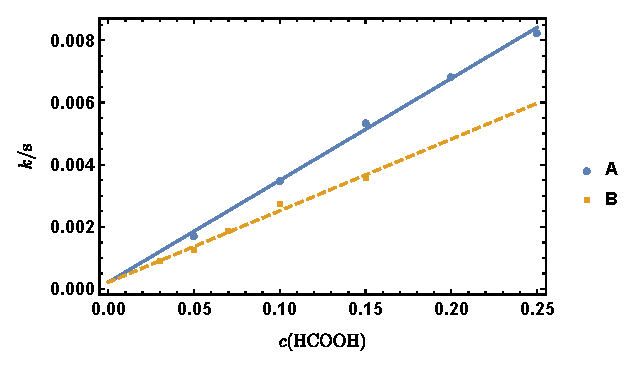
\includegraphics[width=0.48\textwidth]{figures/hcooh.eps}
	\label{hcooh}
}
\subfigure{
	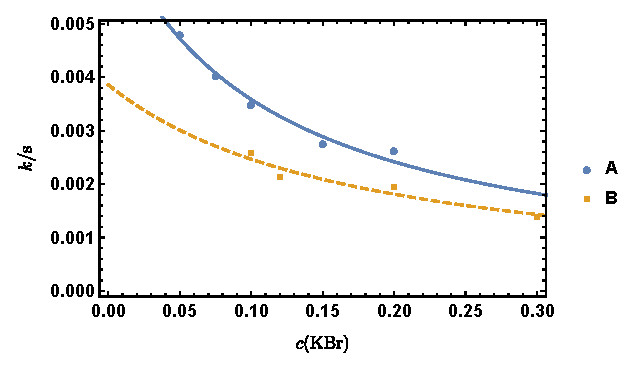
\includegraphics[width=0.48\textwidth]{figures/kbr.eps}
	\label{kbr}
}
\subfigure{
	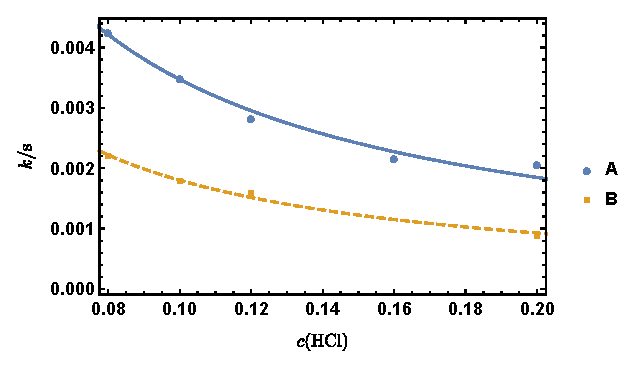
\includegraphics[width=0.48\textwidth]{figures/hcl.eps}
	\label{HCl}
}
\subfigure{
	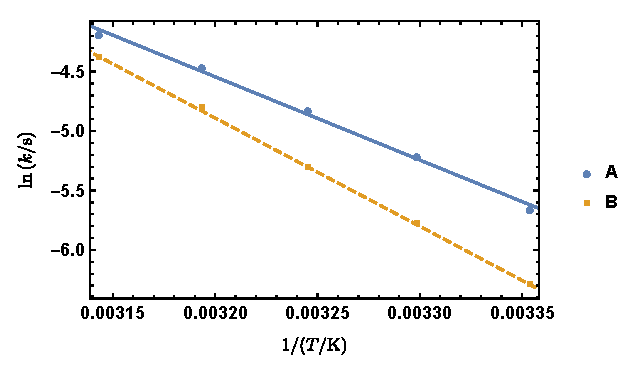
\includegraphics[width=0.48\textwidth]{figures/exptemp.eps}
	\label{temp}
}
\caption{The trends of $k$ towards different variants, among which the data of $c(\ce{KBr})$ and $c(\ce{HCl})$ are fitted by $\frac{C_1}{c/C_2 + 1}$.}
\label{fit}
\end{figure}
\begin{figure}
\centering
\includegraphics[width=0.8\textwidth]{figures/reaction_mechanic.png}
\caption{The proposed mechanism of the oxidation of formic acid by bromine in aqueous solution}
\label{mechanism}
\end{figure}
\begin{figure}
\centering
\includegraphics[width=0.8\textwidth]{figures/process-G.jpg}
\caption{Gibbs free energy curve of the system at different state}
\label{GCurve}
\end{figure}
\begin{figure}
\centering
\includegraphics[width=0.45\textwidth]{figures/TS1-white.png}
\caption{Ball-stick model of the transition state}
\end{figure}
\begin{table}
\centering
\caption{The fitting result of the trends of $k$ towards different variants}
\begin{tabular}{c|ccccc}\hline
& Variant & Fitting Function & $R^2$ \\\hline\\[-1em]
\multirow{6}{*}{A} & $c$(HCOOH) & $k = 0.0327773 c + 2.19794 \times 10^{-4}$ &  0.996417 \\\\[-1em]
& $c$(KBr) & $k= \frac{0.00693094}{1+9.33714 c}$ & 0.998844 \\\\[-1em]
& $c$(HCl) & $k = \frac{0.0284047}{1+ 71.825 c}$ & 0.998414 \\\\[-1em]
& $T$ & $\ln k = - \frac{6999.34}{T} + 17.8541$ & 0.996029	\\\\[-1em]\hline\\[-1em]
\multirow{6}{*}{B} & $c$(HCOOH) & $k = 0.0230375 c + 2.14535 \times 10^{-4}$ & 0.985107 \\\\[-1em]
& $c$(KBr) & $k= \frac{0.00385937}{1+5.64876 c}$ & 0.996225 \\\\[-1em]
& $c$(HCl) & $k = \frac{0.0303935}{1+ 158.798 c}$ & 0.999134 \\\\[-1em]
& $T$ & $\ln k = - \frac{9100.81}{T} + 24.2389$ & 0.999577	\\\hline
\end{tabular}
\end{table}


The experimental data obtained are shown in Table.\ref{data}, with their graphic representation shown in Fig.\ref{fit}. It is
quite evident that there exist a sharp difference between results from the spectrophotometric method and the electrochemistry method. Two factors may contribute to the difference, diffusion and response function, that mainly affect the data from electrochemistry method.

To further elaborate this, we start from the basic equation that describes the diffusion of a substance in the liquid phase to the surface of a solid:
\begin{equation}
	\frac{d c_s}{dt} = k (c_l - c_s)
\label{diffusion}
\end{equation}
where $c_l$ refers to the concentration of the substance in the liquid phase, while $c_s$ the `equivalent' concentration in the solid phase, which can be deduced by the chemical potential of the substance on the surface. Considering that the diffusion of the substance is comparatively small, $c_l$ can be regarded as dominated by chemical reaction, namely
\begin{equation}
	c_l = c' e^{-k't}
\end{equation}
where $c',k'$ are constants. (\ref{diffusion}) can be deduced by assuming the form of $c_s$ as
\begin{equation}
	c_s = \chi(t) e^{-k't}
\end{equation}
which gives
\begin{equation}
\begin{cases}
	\chi(t) = C_1 e^{(k'-k) t} + C_2,\\
	 c_s = \frac{k c'}{k'-k} e^{-k't}(e^{(k'-k)t}-1)
	 \end{cases}
\end{equation}
where $C_1,C_2$ are constants that are replaced using the boundary condition,
\begin{equation}
	c_s \big|_{t=0} = 0
\end{equation}
and infomation from $c_s$.
It reveals the influence of the diffusion in the measurement, the term $e^{(k'-k)t}-1$ being the main delimiter. Smaller $k$ with small sets of $t$ will result in larger deficiency in the measurement of $k'$, which might be the case in the electrochemistry method. It can be partly verified by the experimental result of the trend of $k$ towards the temperature, which indicates a higher activation energy. This can be explained by the contribution of faster diffusion of \ce{Br2} towards the surface of the electrodes.

The non-constant response function of the measurement system might also contribute to the error. The detection of current is achieved through complicated electromagnetic system, which results in non-constant response function. The output function can be regarded as the convolution of the signal function and the response function, namely
\begin{equation}
	P = S * R = \int S(t) R(T-t) \, dt
\end{equation}
where $P$ stands for the output, while $S$ and $R$ for the signal function and the response function, with $T$ defined as the time interval for a measurement. Given that $S$ is a exponential function, it can be readily proved that $P$ is also a exponential function under the same base. A non-constant response function, however, deviates the output function with considerable error, and it is conspicuous that a larger time interval leads to worse data sets. Compared with spectrophotometric method, electrochemistry method is much more likely to suffer from such a factor, w.r.t. its relatively longer measurement of time.

The result of the computational calculation is partially listed in Table.\ref{gascalc},\ref{speciescalc}. Table.\ref{gascalc} reveals the absense of activation energy, which should be attributed to the active property of the ions in the gas phase. Introducing solvent effect, the activation energy calculated is 0.013081 Hartree, which is equivalent to 8.2085 kcal/mol. Experimental data exhibit the activation energy of 
14.48 kcal/mol, which partly verifies the proposed mechanism. The deviation is attributed to many reasons, including decent accuracy of the DFT method (Currently no DFT method can reach chemical accuracy), decent approximation of the solvent effect which ignores the dynamic interaction of the system and the solvent, and neglecting the interaction between reactants, such as two HCOOH molecules. From another perspective, the observed activation energy cannot represent the correct activation energy, mainly because of the various energy state of both the reactants and transition state concerning kinetic energy and electromagnetic energy, occupying serveral cells in the phase space, which leads to distributed activation energy in the practical system.

 Calculation also reveals that there is no tendency of reaction between HCOOH and \ce{Br2}, while the species \ce{Br3-} will react with \ce{HCOO-} and decompose into \ce{Br-} ions simultaneously, requiring much energy that is equivalent to that required for the decomposition of \ce{Br3-} into \ce{Br2} and \ce{Br-} itself. With these results we propose the mechanism whose graphic representation is shown in Fig.\ref{mechanism}.
\section{Conclusions}
Both spectrophotometric method and electrochemistry method verifies the proposed mechanism that \ce{HCOOH} is oxidized by \ce{Br2} through the main reaction of second order between \ce{HCOO-} and \ce{Br2}. Error between two methods is attributed to the diffusion of \ce{Br2} towards the electrode and the response function of the electrochemistry detection system. The activation energy is predicted decently by computational calculation, further denying the possibility of the reaction between neutral \ce{HCOOH} and \ce{Br2}.
\bibliography{References}

\newpage
\section*{Review}
\wuhao
\begin{center}
\xiaosan\textbf{Rise of computational chemistry}

\xiaosi{ Rui Li (3160102098)}
\end{center}
Chemistry was rumored to be a subject that does not require much mathematics- students recite the words in the textbooks and earn a high score without much effort. Empirical laws and outdated equations are listed everywhere, even without an elaboration of why they really are. After years, students find themselves forgotten almost everything, and fail to give a clue on what chemistry is.

As wikipedia puts it, 'Chemistry is often called the central science because of its role in connecting the physical sciences, which include chemistry, with the life sciences and applied sciences such as medicine and engineering.' It has never forgot the roles physical science has taken, but most of the chemistry educators are. They do not acquire a complete system of physical science (especially physics itself), not to mention some basic skills of advanced mathematics. Barely teachers can lecture an orthodox style of quantum mechanics that is based on theoretical dynamics and electrodynamics, or a detailed deduction of the theorems in thermostatistics.

However, chemistry is stepping into a new era- computational chemistry has gained enormous progress owing itself to the development of computers. Quantum mechanics is no longer an inaccessible resource for chemists, while molecular dynamics is becoming a must for chemical researches. With these technologies available, chemistry can finally revolutionalize itself to a more sophisticated and rational subject. Moreover, algorithms and coding skills are emphasizing their importance in everyday researches w.r.t. the recent application of machine learning in organic chemistry.

Nevertheless, the curriculum designed for chemistry-majored students are outdated compared with the trends - unsatisfying curriculum for quantum mechanics and thermostatistics, no lectures for programming in chemistry, far too little requirement for methematical skills. In these experiments only the process is emphasized, with too little mention to the physical background and a motivation set for students to investigate the mathematical or physical deduction of the phenomena. Further, the availability of the original data with the ability to process a mass of them is a fundamental requirement in the researches- no researchers will just print the graphs with several points chosen to form the experimental data.

The era of predominating experiments with empirical laws has gone; an era of sophisticated deductions with fascinating programs is coming.


\newpage
\begin{center}
\xiaosan\textbf{Comments on the experiment}

\xiaosi{Yiliu Li}
\end{center}
We studied the kinetics of the oxidation of formic acid by bromine in aqueous media, using both spectrophotometric method and electrochemistry method. This research experiment is a new experiment to us, which is a little bit tough and unfamiliar to us, thus requiring a lot of time.

I, together with Zongwei, used electrochemistry method. Although there are some procedures on the book, we still need to consider the uniformity of our two methods. After careful consideration and systematical design, we chose several variables and concentrations of the solutions. 

Even though we have used the electrochemistry method before, there are many details that we should pay attention to. Due to the special quality of the machine, we have to save the data every time we finish taking them. Unfortunately, we forgot to save the data on the computer at the first two times. Oh my god! When we first realized it, we were so shocked and upset because it took us a lot of time to take the data. On the other hand, we realized this before we began to do the third experiment, which is not that awful.This accidental experience is a little bit ridiculous, but it also teaches us that we should always keep in mind to save the data!!!

Our group has five members, they are very helpful and we cooperate well with others, so even though we forgot to save the data first, we were still the first to finish the experiment. My partners really did a good job and I learn a lot from them.
\newpage
\begin{center}
\xiaosan\textbf{从``探究性实验''浅谈化学实验改革}

\xiaosi{ 黄宗玮 (3160104940)}
\end{center}

在上周做实验之前,我还是按照常规操作写完了预习报告,然后就秦同学就突然找我说,探究性实验要不要一起组队。我当时吓了一跳,探究性实验不是应该提前准备,查阅相关文献,自行设计实验方案的吗?明天就做实验了,文献好说,但是仔细看和另行设计方案肯定是来不及了(主要是我认为探究性实验不仅要能重复前人的工作,也一定要有自己的特点。即重复+创新)。但是秦说老师已经给了除了书上的方案的另一种方案(都怪我平时不水群),因此我稍微看了一下(毕竟我已经了解了书上的方案了),大概明白了这个方案2要怎么操作,但是还是觉得所谓‘探究性实验’,就按照书上和老师给出的方案未免还是陷入了只有‘重复’而没有‘创新’的情况。因此我和同寝室的李睿商量了一下,这个‘探究’要怎么玩(他可是玩实验的行家),他本来还是想用他之前的电化学扩散模型(因为方案1就是电化学法),但是我跟他说这个不够‘化学’,这个实验的重点还是化学反应动力学和反应机理,玩这个东西目前最好的理论还是过渡态理论。最后商量的结果是用Gaussian研究反应机理和活化能。

但是我们万万没想到的是,事实证明,李睿最初的扩散模型的想法在误差分析中十分重要,因为我们发现了电化学法和光谱法的结果存在的系统误差,这个误差经过分析后被认为是由于电化学需要扩散和平衡过程导致的,而定量描述这个误差就需要他提到的扩散模型。遗憾的是,由于时间问题,我们并没有对这个误差进行具体的模拟,只是用了一些比较普适的方程来描述,这也是本次实验稍微有些遗憾的地方。

下面来谈一谈从这次实验窥见的问题。

首先是时间问题,个人认为如果希望通过这个‘探究性实验’培养同学们的科研思维,首先就是要给同学们足够的自由空间,而实现这样一个自由空间的非常重要的一点就是拥有足够的时间和实践想法的设备(软资源+硬资源)。本次的实验一个很明显不足的就是时间不够,拿不出三节课至少也要有两节实验课的时间,比如像中化一那样,一节课的时间根本没有分析数据——提出猜想——补充实验——证实或证否或修正这样的feedback过程,这样的不过是“大一些的普通实验”。

另外一个东西就是思维的局限性,在这样的一个‘探究’为主的实验中应该将书上以及相关文献作为“参考”而不是“指南”,一个班里13个人,3个组,应该每个组都能拿出来自己独特的地方(这里不得不提一句,王永尧老师已经为我们创造了足够宽松和开放的氛围),不要将自己的思维被所谓的“文献”限制,别人做地再好也只不过是个参考,因此我们也是希望通过自己的行动来为这个实验增加一些‘探究’的氛围(有些人片面地将其理解为“恶性竞争”,个人不以为然,这是科研思维培养的必由之路,此时不练,更待何时?)。

另外谈一点关于基于计算的理论化学的东西。

随着现在计算机技术的发展,当代的化学家必须认识到在这样一个算力极大提高的时代,之前很多在理论上不能被处理的东西变得可以理解了,而且在中化2中加入的基于商业软件的DFT相关理论的应用也证实了我的想法。所以,鼓励学生走“理论+实验”的方法研究问题私以为是之前的化学家梦寐以求甚至想都没想过的事情,而且从本科就培养这样的思想,会对大家对化学现象背后的本质加深认识。

\newpage
\begin{center}
\xiaosan\textbf{在实验中锻炼技能,在探究中历练自我}

\xiaosi{秦宇轩(3160103768)}
\end{center}

一直很喜欢伽利略的一句话:“科学的真理不应该在古代圣人的蒙着灰尘的书上去找,而应该在实验中和以实验为基础的理论中去找。真正的哲学是写在那本经常在我们眼前打开着的最伟大的书里面的,这本书就是宇宙,就是自然界本身,人们必须去读它。”每每回味起中级化学实验2课程中关于甲酸氧化动力学实验的探究,我都感触颇深。

和此前的化学分析实验、无机化学实验、有机合成实验、仪器分析实验不同,物理化学实验综合了化学领域中各分支所需要的基本实验工具和研究方法,通过应用物理学的原理与技术,使用某个仪器或若干仪器组合成的测量体系,对系统的某一物理化学性质进行测量,进而研究化学问题。而化学科研的很多问题的解决正是立足于这些性质,可见物理化学实验的研究方法和实验技能是化学工作者所必备的基本功,这次物理化学实验的探究性学习更能锻炼这方面的个人能力。  

本次实验内容是用电动势法和光密度法分别探究甲酸被溴氧化反应的动力学,除了需要测定反应对各种实验物质的反应级数、速率方程中的速率常数以确定速率方程,还需要计算反应的活化能以及根据速率方程推导该反应的机理,工作量较大。我和吴冠履同学主要负责光密度法实验,实验伊始我们就遇到了问题,虽然相关浓度对照组的设置按照参考文献和实际条件进行了换算,但是测得的吸光度竟然高达1.4,为了排查这个问题,我们耗费了不少溶液和时间,最终发现该分光光度计的光路存在故障。尽管仪器的故障让前期的诸多准备工作白白浪费,但我们并没有为之抱怨,而是通过不断熟练的操作和配合提高实验效率。测量操作中我们也遇到了一些考验,印象最深的是我们需要将实测实验组所属的两瓶溶液混合倒入反应烧杯中,充分混合均匀一段时间再倒入比色皿中。但这个时间很难把控,混合时间过短,混合不均匀,所得数据会因局部浓度差异产生误差;若混合时间过长,对于高浓度、高温度反应组而言,反应速度过快,后续记录的实验点可能会降低到浓度吸光度的线性范围之下,使得可靠的实验数据减少,对于这个问题,我们只能通过反复多次实验,改善不理想的实验组,从最终的分析结果可以看出,拟合程度达到了我们的预期,也成功预测了相关反应的动力学方程和反应级数。事实上,只有多遇到困难和问题,才能在坎坷挫折和历练中升华自己,失败是科研者的家常便饭,学会利用失败剖析则是科研者必备的素质。然而尽管光密度法在操作上有其简便性,但其可控性、精密度等方面不如电化学法,对于颜色的要求也导致该方法适用范围较窄,相关应用的文献资料较少。相较另一种电化学方法,我们在最终的分析中也指出,两种方法的差异主要源于溴相对于电极的扩散和本实验电化学检测系统的响应函数。表征动力学实验中浓度随时间的变化有很多方法,电导、电动势、吸光度、折射率、蒸气压、黏度等都可以作为我们解决问题的有力武器,如何选择最合适的方法或是探索出适用性不同的新方法,也是值得我们总结并在今后的科研道理上深加体会的。

此外,这次探究实验是我们五个同学一个小组的团队实验,团队顾名思义是为了实现某一目标而由相互协作的个体所组成的正式群体。基础学科的科研需要团队协作精神,当团队合作是出于自觉和自愿时,它必将会产生一股强大而且持久的力量。本次实验从设计、讨论,到实验、操作,到分析、拟合,都是通过我们小组的明确分工与通力配合才实现较为圆满的结果,不像其他探究实验,本次实验操作过程相对比较繁琐,需要更多密切的配合,考验了我们的统筹规划能力与团队协作能力。

在探究中锻炼了技能,在分析中历练了自我。本次实验我获益颇丰。

\newpage
\begin{center}
\xiaosan\textbf{心得感言}

\xiaosi{吴冠履 (3160100087)}
\end{center}
化学反应的动力学研究是一个重要的对反应进行方面的实验方法,在这次实验,我们测试的是甲酸氧化的反应动力学,再对这一种一级反应的动力学测出速率常数的方法有很多,而实验中所用的方法有两种,一是分光亮度法,我们藉由溴与甲酸发生氧化反应后的颜色改变从而对其吸收度改变,以Lambert-Beers law来作图后推导出反应速率常数;其二则是电动势法,立用反应实时的电动势监控,同样地,推测出了这个反应的速率常数。

这次,我们最主要的研究项目是反应速率,反应速率是化学反应快慢程度的量度,广义地讲是参与反应的物质的量随时间的变化量的绝对值,分为平均速率与瞬时速率两种。平均速率是反应进程中某时间间隔内参与反应的物质的量的变化量,可用单位时间内反应物的减少量或生成物的增加量来表示;瞬时速率是浓度随时间的变化率,即浓度-时间图像上函数在某一特定时间的切线斜率。用实验方法测定反应速率受反应物量或浓度影响的定量方程称为速率方程,速率方程中各浓度的指数称为相应物质的反应级数,它们的和称为「总反应级数」,也可简称「反应级数」。反应的级数是不能由化学方程式的类型推断的,常见的级数反应如零级反应、一级反应、二级反应,都会有各自不同的速率方程。速率方程中的常数k称为速率常数,可看作单位浓度下的反应速率。建立速率方程时一般采取两种方法:作图法与初速法。控制化学反应速率是许多实践活动的需要。绝大多数化学反应的速率都是随着反应进行而不断减慢的,并且同一反应,在不同浓度、温度、压力、相态下,是否使用催化剂以及使用不同的催化剂,都会对反应速率造成不同的影响。

回到实验的手段方面,基于在反应物质方面,我们是没有办法直接地测试出反应的每一个时刻的物质消耗量,所以,势必要找到一些在反应当中,会随着反应的进程中物质变化量的物理、化学性质,也就是实验中测量的吸亮度及电动势,而发现这些性质,乃是前人的累积,当今对于动力学的测试方面,有相当多的发展,令人叹为观止。

本次实验中,我执行的实验室分光亮度法的测试。这个方法的操作其实是相当地容易,因为在提供的实验方案中,已经有详细地给出了仪器所需要的最大吸收波长以及实验的方法,我们唯一要做的事情是,设计好测试的浓度。与实验方案较为不同的是,这次我们使用的仪器并不需要自己进行祭时,这个方面大大地减少操作上的误差,不过在混合不同溶液方面,还是希望有更好的方法达成直接混合后测试。

一般来说,在化学的理论课上,对于动力的讨论不少,在本次实验中,很惊人地,我发现到,实验方面对于理论的一个条件都是需要进行相当多得考虑,在本次实验后,能更加清楚地理解化学反应动力学的理论及实验方法。

\end{document}
